\documentclass[a4paper,12pt]{article}
\title{\textbf{Bioimpresi\'{o}n 3d aplicada al campo Card\'{i}aco}\\\large{ECB, EMDTB, SHB || Q6 EEBE - UPC}}
\author{Oriol Ruiz Dom\'{i}nguez}

\usepackage{mathtools}
\usepackage{hyperref}
\usepackage[utf8]{inputenc}
\usepackage{lmodern}
\usepackage[spanish]{babel}
\usepackage[left=1.5cm,top=2.5cm,right=1.5cm,bottom=2.5cm]{geometry} 
\usepackage{amsmath,amssymb,amsthm,textcomp}
\usepackage{graphicx}
\usepackage{eurosym}
\usepackage{listings} 
\providecommand{\abs}[1]{\lvert#1\rvert}
\usepackage{color} %red, green, blue, yellow, cyan, magenta, black, white
\definecolor{mygreen}{RGB}{28,172,0} % color values Red, Green, Blue
\definecolor{mylilas}{RGB}{170,55,241}

%Extra levels of subsection
\usepackage{titlesec}
\setcounter{secnumdepth}{4}
\titleformat{\paragraph}
{\normalfont\normalsize\bfseries}{\theparagraph}{1em}{}
\titlespacing*{\paragraph}
{0pt}{3.25ex plus 1ex minus .2ex}{1.5ex plus .2ex}

\begin{document}
\maketitle
\pagebreak
\tableofcontents
\pagebreak
\listoffigures
\pagebreak


\pagebreak
\section{Introducción}

\pagebreak
\section{Historia}

\subsection{Historia de los biomateriales}

\subsection{Historia de la impresión y bioimpresión 3D}

\subsection{Biomateriales e impresión 3D en el campo vascular}

\pagebreak
\section{Marco actual - Investigación y mercado}

\pagebreak
\section{Marco legal - Nivel de mercado. Normativa}

\pagebreak
\section{Fisiología}

\subsection{El sistema circulatorio}

\subsection{El corazón}

\subsubsection{Función del corazón}

\subsubsection{Anatomía del corazón}

\subsubsection{Actividad eléctrica del corazón (Potenciales de acción cardíacos)}

\subsubsection{Mecanismo de contracción cardíaco}

\subsubsection{Ciclo cardíaco}

\subsection{Problemas y enfermedades cardíacas}

\pagebreak
\section{Biomateriales y Biocompatibilidad}

\subsection{Principales materiales para bioimpresión}

\subsubsection{Cerámicos}

\subsubsection{Polímeros}

\subsubsection{Metales}

\subsubsection{Hidrogeles}

\subsection{Biocompatibilidad}

\subsection{Ventajas e inconvenientes de los biomateriales}

\subsection{Impresión de stents}

\subsubsection{Metodología}

\subsubsection{Materiales empleados}

\subsubsection{Ventajas e inconvenientes de Stents 3D}

\pagebreak
\section{Bioimpresión}
\subsection{Estrategias de bioimpresión}
La bioimpresión se basa en la deposición de material biológico siguiendo un patrón establecido. Existen variedad de métodos que cumplen este objetivo, aunque los principales son: por inyección de tinta, mediante microextrusión o bien mediante un láser.

	\begin{figure}[!ht]
	\begin{center}
	  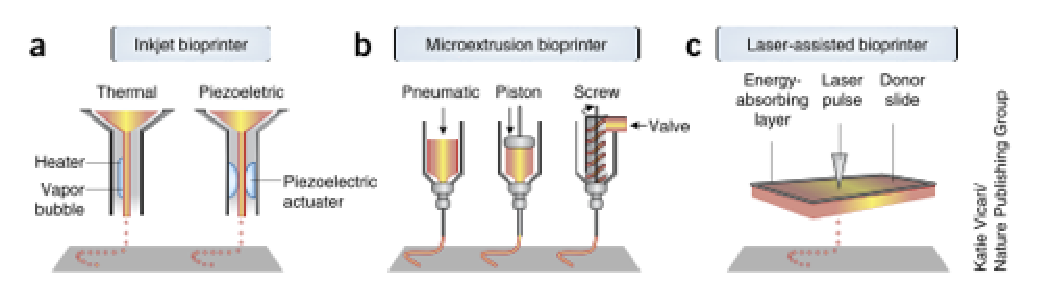
\includegraphics[width=0.5\textwidth]{Figuras/tiposBioimpresion.eps}
	  \caption{\emph{Estrategias de bioimpresión. }Extraído de \emph{---FALTA CITAR---}.}
	\end{center}
	\label{tiposBioimpresion}
	\end{figure}

\subsubsection{Inyección de tinta}
Las impresoras de inyección de tinta son el modelo más empleado en el ámbito no biológico. De hecho, las primeras bioimpresoras de inyección de tinta se crearon a partir de la modificación de impresoras comerciales. Su funcionamiento consiste en la deposición de un volumen de tinta controlado en la posición establecida.

Para realizar la eyección de tinta hay dos métodos: térmica y acústicamente.

\paragraph{Inyección térmica}
El método térmico consiste en calentar eléctricamente el cabezal entre 200 y 300 grados para realizar pulsos de presión y que caiga el material. Estudios han demostrado que esta temperatura, al producirse en alrededor de 2$\mu s$ y estar tan localizada, no tiene gran impacto en la estabilidad de las moléculas biológicas, como el ADN ya que solo provocan un incremento de entre 4 y 10 ºC.


\paragraph{Inyección acústica}
Otra manera de realizar inyección de volumen de líquido controlado es mediante un cristal piezoeléctrico. Al aplicarle un voltaje a este piezoeléctrico este produce una onda acústica, así como un cambio rápido en su forma de manera que genera la presión suficiente como para eyectar el líquido. También es posible realizar la presión mediante una fuerza de radiación acústica asociada a los ultrasonidos.

Varios parámetros como el pulso, la duración o la amplitud se ajustan para controlar el volumen de eyección y la frecuencia a la que se producen.

\subsubsection{Microextrusión}

\subsubsection{Láser}

\subsection{Impresoras}
El mercado actual de impresión 3d está creciendo exponencialmente dado al reducido precio al que se ha conseguido diseñar los equipos. Hay diferentes empresas destinadas al sector, aunque hay que hacer una mención especial a las impresoras diseñadas en la plataforma open-source reprap.org, en la cuál se puede encontrar un ámplio abanico de diseños de manera gratuita.

Uno de los modelos más fabricados es la impresora Prusa I3 bajo la licencia de reprap, diseñada por el CEO de PrusaResearch Josef Průša. Dada la facilidad de acceso a las diferentes partes del equipo y la posibilidad de cambiar sus partes, estos modelos han sido empleados por muchas empresas tanto para ser comercializados como para la creación de impresoras adaptadas para realizar bioimpresión.

Más allá de las impresoras open-source, empresas como BCN3D (bajo la FundacióCIM-UPC), han desarrolado impresoras como la BCN3D Sigma. De nuevo, los modelos básicos no suelen estar diseñados para realizar bioimpresión, pero en laboratorios como el del Dr Gioseppe Scionti realizan la adaptación para ello.

\subsubsection{Partes básicas}
Todos los modelos más comerciales de impresoras 3d cuentan con unas especificaciones similares. Es necesario es necesario tener un cabezal de impresión (habitualmente extrusor), una superficie de soporte (habitualmente cama caliente), servomotores (habitualmente 5), una placa controladora y la estructura.

Para poder realizar una impresión 3d es necesario tener movimiento en 3 ejes (x, y, z). Los diferentes modelos de impresión suelen diferir en qué se mueve de la impresora (el cabezal, el soporte…), pero el modelo generalizado realiza movimiento del cabezal en los ejes x (un servomotor) y z (dos servomotores), mientras que para el eje y se mueve el soporte (un servomotor). El servomotor restante es el que controla la cantidad de material a poner en el modelo.

	\begin{figure}[!ht]
	\begin{center}
	  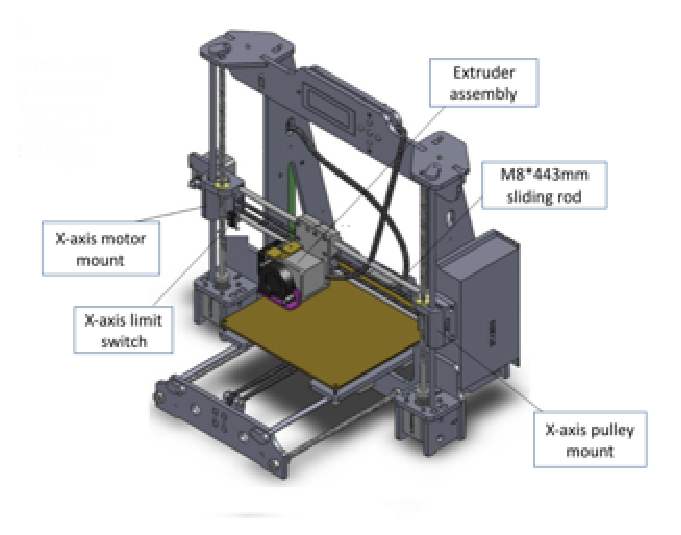
\includegraphics[width=0.5\textwidth]{Figuras/partesImpresora.eps}
	  \caption{\emph{Partes de una impresora. }Extraído de \emph{Manual de montaje Tronxy P802MA}.}
	\end{center}
	\label{partesImpresora}
	\end{figure}

%\paragraph{Adaptación para impresión de Stents}


%\subsubsection{Preparación}

%\subsubsection{Preimpresión}


\subsection{Modelado}
Otro pilar esencial cuando se habla de impresión 3D son los modelos que se emplean. Estos pueden ser muy diferentes, siendo así su método de obtención totalmente distinto en función de qué estemos buscando. Habitualmente se crean modelos directamente desde un ordenador, con programas como \emph{Solidworks} o \emph{Autodesk Fusion} para modelos mecánicos o bien \emph{Blender} o \emph{3Ds Max} para figuras más gráficas.\\

Por otro lado, en el ámbito de la bioimpresión trataremos más habitualmente con diseños que en vez de crearse desde cero parten de una base: el paciente. Pueden obtenerse imágenes médicas mediante TACs, Resonancias Magnéticas o Angiografías, y a partir de estas crear el modelo del individuo de estudio. Por esta razón, diferenciamos entre el proceso para obtener un modelo de corazón o bien de stent cardíaco.\\

\subsubsection{Modelado cardíaco}
\emph{Nota: el proceso aquí descrito no es necesariamente el mejor ni el más rápido, sinó el que se ha considerado mejor y más optimizado. Existen programas que crean el modelo .stl directamente desde imagenes DICOM, pero han sido rechazados en este trabajo debido a la falta de rigurosidad a la hora de analizar la validez de los datos.}\\

Habiendo realizado la adquisición de datos de nuestro paciente, es muy habitual recibir imagenes en formato DICOM. Para visualizar estas imagenes es necesario contar con un software que visualice los archivos y sea capaz de crear una reconstrucción a partir de las capturas de las diversas capas. Para dicha tarea destaca el software \href{http://www.osirix-viewer.com/}{OsiriX}, mediante el cual podremos obtener la imagen 3D en un formato \empn{.wrl}.\\

A partir de aquí comienza el proceso más complicado del modelaje cardíaco 3D. Las imagenes obtenidas cuentan con diversidad de impurezas, las cuales pueden ser desde errores en la obtención o el procesado hasta tejido duro indeseado. Es por ello que se realiza una fase de limpieza y suavizado del modelo. Un programa que nos permite hacer esta tarea es \href{https://www.blender.org/}{Blender}, el cual es un programa Open Source en 3D ya que permite crear modelos, animaciones, renderizar, crear vídeos o incluso juegos. Además, nos permite abrir nativamente el formato de archivo .wrl sin necesidad de realizar ningún tipo de conversión.\\

Teniendo abierto el archivo de corazón con todos los elementos que lo rodean en Blender, deberemos seleccionar todas las partes indeseadas y pulsar X para eliminarlas.\\

Para poder quitar imperfecciones que se hayan generado al combinar las imagenes de las diferentes capas, se aconseja realizar un suavizado del propio modelo. Este proceso también se puede realizar con Blender seleccionando las caras que se quieren suavizar y aplicando la opción \emph{Shading Smooth}.\\

Pese a todo, a veces no nos interesa realizar la impresión 3D de todo el modelo, pero queremos contar con todo para el trabajo anterior sobre el ordenador. En este caso, realizar un proceso de segmentación es la opción más correcta. Mediante programas como \href{https://www.rhino3d.com/}{Rhinoceros} se pueden diferenciar capas dentro de un mismo modelo, y empleando la opción \emph{Mesh Split} se puede dividir el modelo en partes y asociarlo a las capas creadas anteriormente. De esta manera, podemos aplicar diferentes colores en función de la capa y ver, por ejemplo, partes oxigenadas y partes desoxigenadas del mismo modelo de forma clara.\\

	\begin{figure}[!ht]
	\begin{center}
	  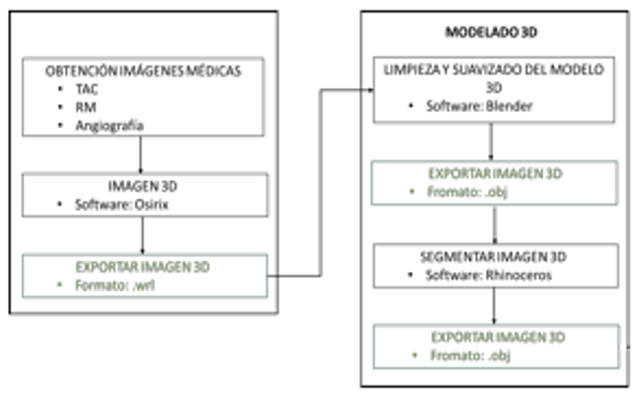
\includegraphics[width=0.5\textwidth]{Figuras/modeloCardio.png}
	  \caption{\emph{Proceso propuesto de modelado cardíaco}}
	\end{center}
	\label{modeloCardio}
	\end{figure}

\subsubsection{Modelado de Stents}
De una manera muy diferente se crean los modelos de Stents. Teniendo en cuenta las adaptaciones que deben tenerse en cuenta para imprimirlos, el proceso de diseño no seguirá un modelo que se visualice fácilmente.\\

En primer lugar deberemos considerar 




\pagebreak
\section{Práctica}
\subsection{Impresión de Stents}
\subsection{Simulación de impresión}
\subsection{Propuestas de mejora}



\pagebreak
\section{Proyección}

\pagebreak
\section{Conclusiones}


\pagebreak
\section{Bibliografía}


\pagebreak
\section{Anexos}

\end{document}
